\documentclass{article}

\usepackage{amsmath,amssymb}
\usepackage{tikz}
\usepackage{pgfplots}
\usepackage{xcolor}
\usepackage[left=2.1cm,right=3.1cm,bottom=3cm,footskip=0.75cm,headsep=0.5cm]{geometry}
\usepackage{enumerate}
\usepackage{enumitem}
\usepackage{marvosym}
\usepackage{tabularx}

\usepackage{listings}
\definecolor{lightlightgray}{rgb}{0.95,0.95,0.95}
\definecolor{lila}{rgb}{0.8,0,0.8}
\definecolor{mygray}{rgb}{0.5,0.5,0.5}
\definecolor{mygreen}{rgb}{0,0.8,0.26}
\lstdefinestyle{java} {language=java}
\lstset{language=java,
	basicstyle=\ttfamily,
	keywordstyle=\color{lila},
	commentstyle=\color{lightgray},
	stringstyle=\color{mygreen}\ttfamily,
	backgroundcolor=\color{white},
	showstringspaces=false,
	numbers=left,
	numbersep=10pt,
	numberstyle=\color{mygray}\ttfamily,
	identifierstyle=\color{blue},
	xleftmargin=.1\textwidth, 
	%xrightmargin=.1\textwidth,
	escapechar=§,
	breaklines=true,
	postbreak=\mbox{\space}
}

\usepackage[utf8]{inputenc}

\renewcommand*{\arraystretch}{1.4}

\newcolumntype{L}[1]{>{\raggedright\arraybackslash}p{#1}}
\newcolumntype{R}[1]{>{\raggedleft\arraybackslash}p{#1}}
\newcolumntype{C}[1]{>{\centering\let\newline\\\arraybackslash\hspace{0pt}}m{#1}}

\newcommand{\E}{\mathbb{E}}
\DeclareMathOperator{\rk}{rk}
\DeclareMathOperator{\Var}{Var}
\DeclareMathOperator{\Cov}{Cov}

\title{\textbf{Softwaretechnologie, Übung 13}}
\author{\textsc{Henry Haustein}}
\date{}

\begin{document}
	\maketitle
	
	\section*{Aufgabe 1}
	\begin{enumerate}[label=(\alph*)]
		\item (Analyse-)Verhaltenszustandsmaschine
		\begin{center}
			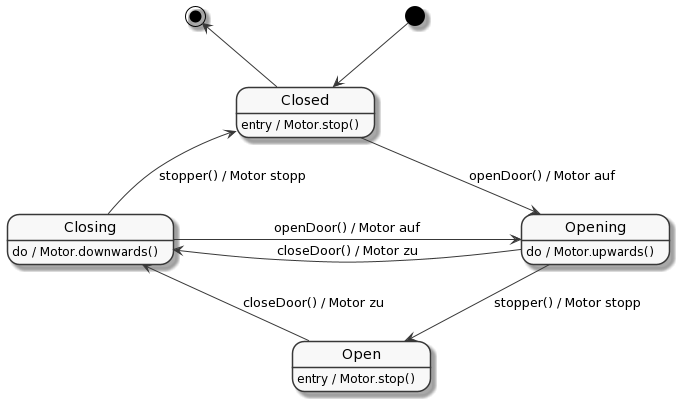
\includegraphics[width=0.50\textwidth]{./Aufgabe13_1a}
		\end{center}
		\item Entwurfs-Klassendiagramm mit State-Entwirfsmuster
		\begin{center}
			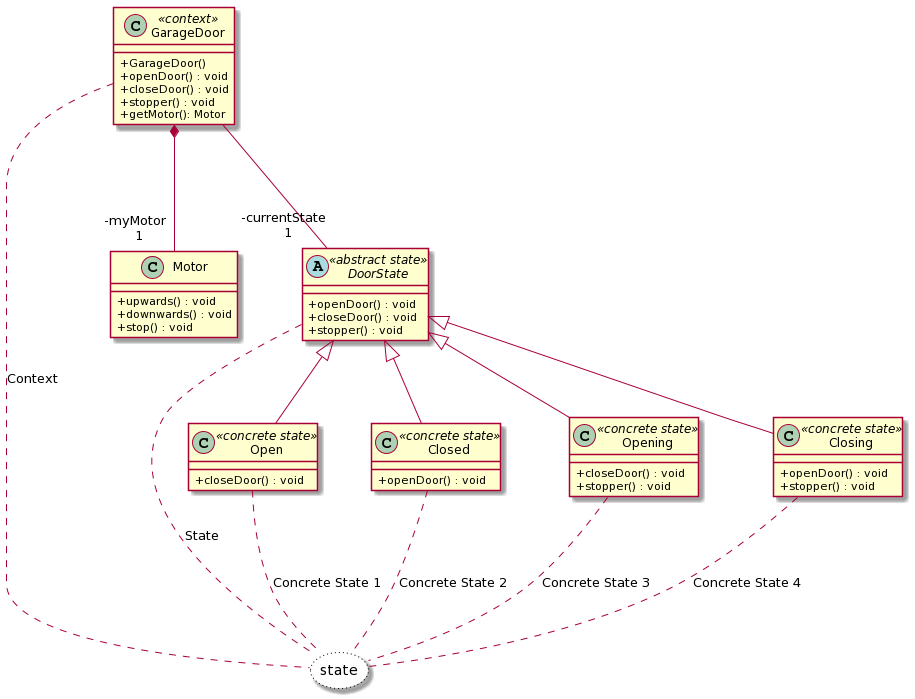
\includegraphics[width=0.50\textwidth]{./Aufgabe13_1b}
		\end{center}
		\item Datei \texttt{GarageDoor.java}
		\begin{lstlisting}[style=java,tabsize=2]
public class GarageDoor {
	private DoorState currentState; 
	private Motor myMotor; 

	public GarageDoor() {
		this.currentState = new Closed();
		this.myMotor = new Motor();
	}

	public void openDoor() {
		this.currentState.openDoor();
	}

	public void stopper() {
		this.currentState.stopper();
	}

	public void closeDoor() {
		this.currentState.closeDoor();
	}

	public Motor getMotor() {
		return this.myMotor; 
	}

	public void setState(DoorState newState) {
		if(newState == null){
			throw new NullPointerException();
		}
		this.currentState = newState;
	}


	abstract class DoorState {
		public void openDoor() {
			throw new IllegalStateException();
		}

		public void closeDoor() {
			throw new IllegalStateException();
		}

		public void stopper() {
			throw new IllegalStateException();
		}
	}

	class Closed extends DoorState {
		@Override 
		public void openDoor() {
			myMotor.upwards();
			setState(new Opening());
		}
	}

	class Opening extends DoorState {
		@Override
		public void closeDoor() {
			myMotor.downwards();
			setState(new Closing());
		}

		@Override
		public void stopper() {
			myMotor.stop();
			setState(new Open());
		}
	}

	class Open extends DoorState {
		@Override
		public void closeDoor() {
			myMotor.upwards();
			setState(new Closing());
		}
	}

	class Closing extends DoorState {
		@Override
		public void openDoor() {
			myMotor.upwards();
			setState(new Opening());
		}

	@Override
		public void stopper() {
			myMotor.stop();
			setState(new Closed());
		}
	}
}
		\end{lstlisting}
		Datei \texttt{Motor.java}
		\begin{lstlisting}[style=java,tabsize=2]
public class Motor {
	public void upwards() {
		System.out.println("Door goes up!");
	}
	
	public void downwards() {
		System.out.println("Door goes down!");
	}

	public void stop() {
		System.out.println("Moving completed!");
	}
}
		\end{lstlisting}
	\end{enumerate}

	\section*{Aufgabe 2}
	\begin{enumerate}[label=(\alph*)]
		\item aUML:
		\begin{center}
			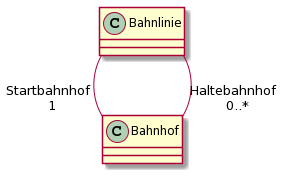
\includegraphics[width=0.5\textwidth]{./Aufgabe13_2a1}
		\end{center}
		dUML (Sichtbarkeiten, Java-Datentypen, gerichtete Assoziationen, Konstruktoren, getter, setter, Parameter, Rückgabetypen von Methoden):
		\begin{center}
			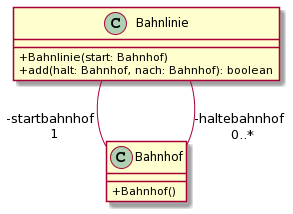
\includegraphics[width=0.5\textwidth]{./Aufgabe13_2a2}
		\end{center}
		jUML (Unterscheidung zw. Klassen und Interfaces, konkrete Java-Implementierungen (hier java.util.List)):
		\begin{center}
			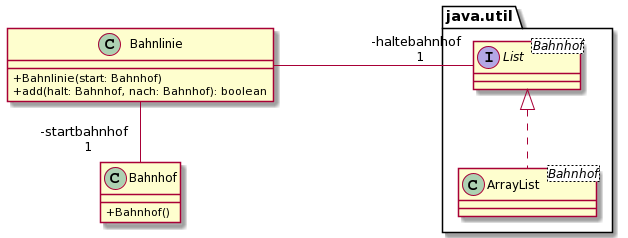
\includegraphics[width=0.75\textwidth]{./Aufgabe13_2a3}
		\end{center}
		\item aUML:
		\begin{center}
			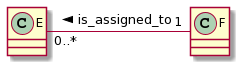
\includegraphics[width=0.4\textwidth]{./Aufgabe13_2b1}
		\end{center}
		dUML:
		\begin{center}
			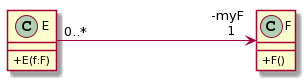
\includegraphics[width=0.4\textwidth]{./Aufgabe13_2b2}
		\end{center}
		Quelltext:
		\begin{lstlisting}[style=java,tabsize=2]
class E {
	private F myF;

	public E (F myF) {
		if(F == null){
			throw new NullPointerException("Gib F du Null!");
		}
		myF = myF;
	}
}
		\end{lstlisting}
		\item aUML:
		\begin{center}
			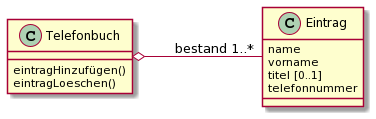
\includegraphics[width=0.5\textwidth]{./Aufgabe13_2c1}
		\end{center}
		dUML:
		\begin{itemize}
			\item Qualifizierte gerichtete Assoziation mit dem Qualifier Telefonnummer $\to$ Multiplizität ändert sich auf 1 (Telefonnummer soll Schlüssel sein).
			\item Qualifizierte gerichtete Assoziation mit dem Qualifier Name $\to$ Multiplizität bleibt bei 1…*, weil es verschiedene Personen mit gleichem Namen aber unterschiedlicher Telefonnummer gibt.
		\end{itemize}
		\begin{center}
			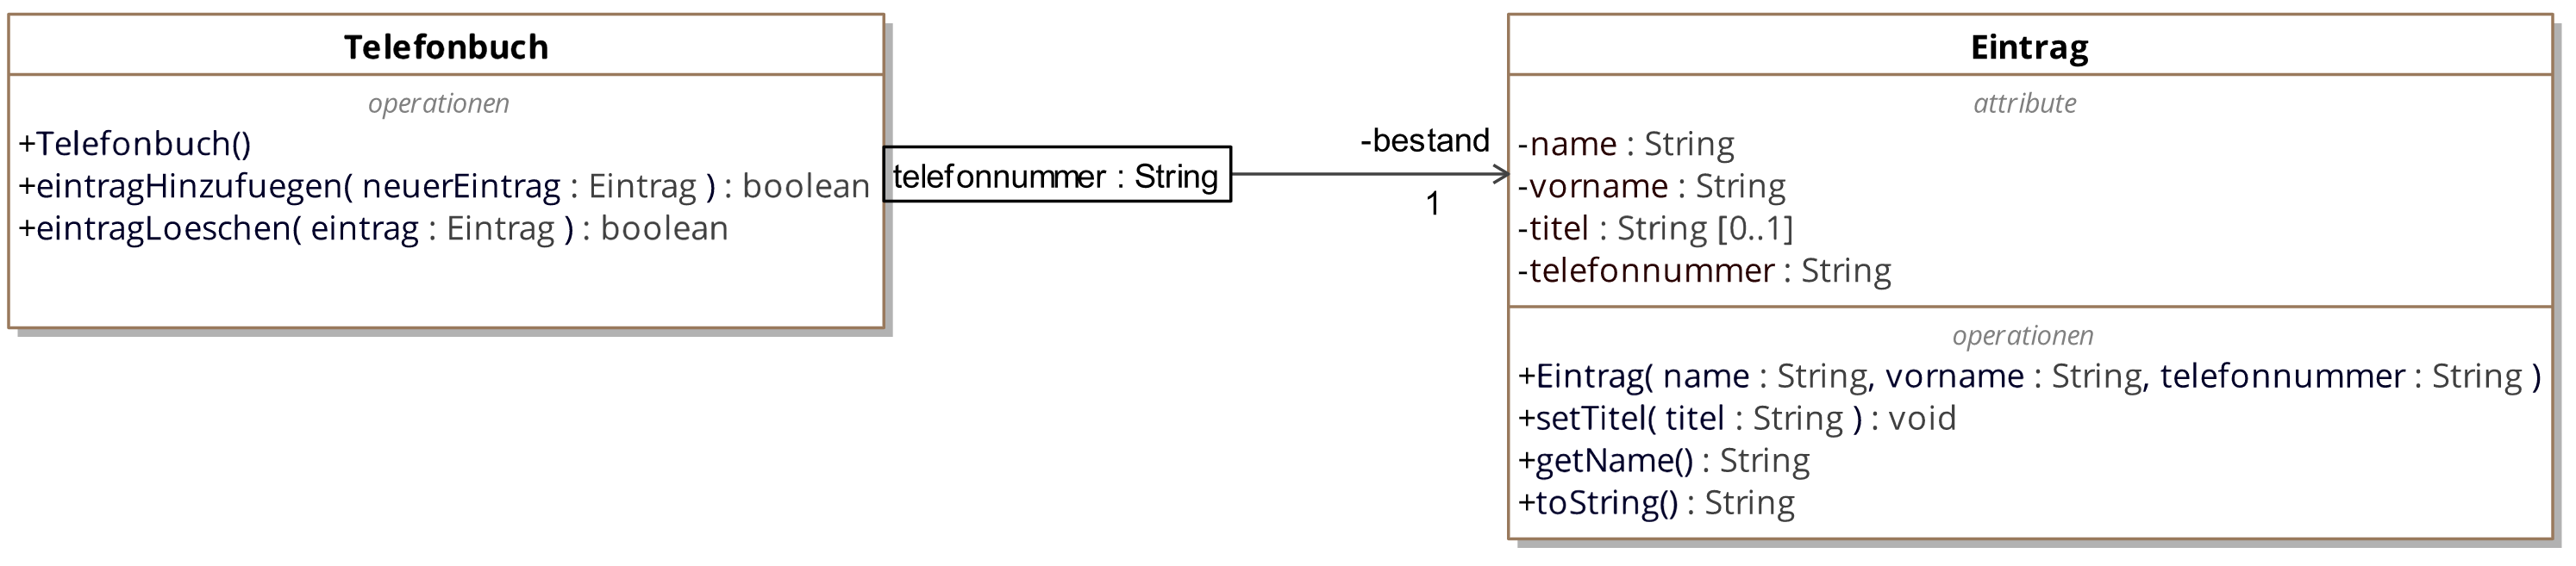
\includegraphics[width=0.75\textwidth]{./Aufgabe13_2c2}
		\end{center}
		jUML (qualifizierte Assoziation als \texttt{Map<key, value>} implementieren, key ist der Qualifier und value sind die zugeordneten Objekte):
		\begin{itemize}
			\item Zu jeder Telefonnummer (Qualifier) genau ein Eintrag zugeordnet.
			\begin{center}
				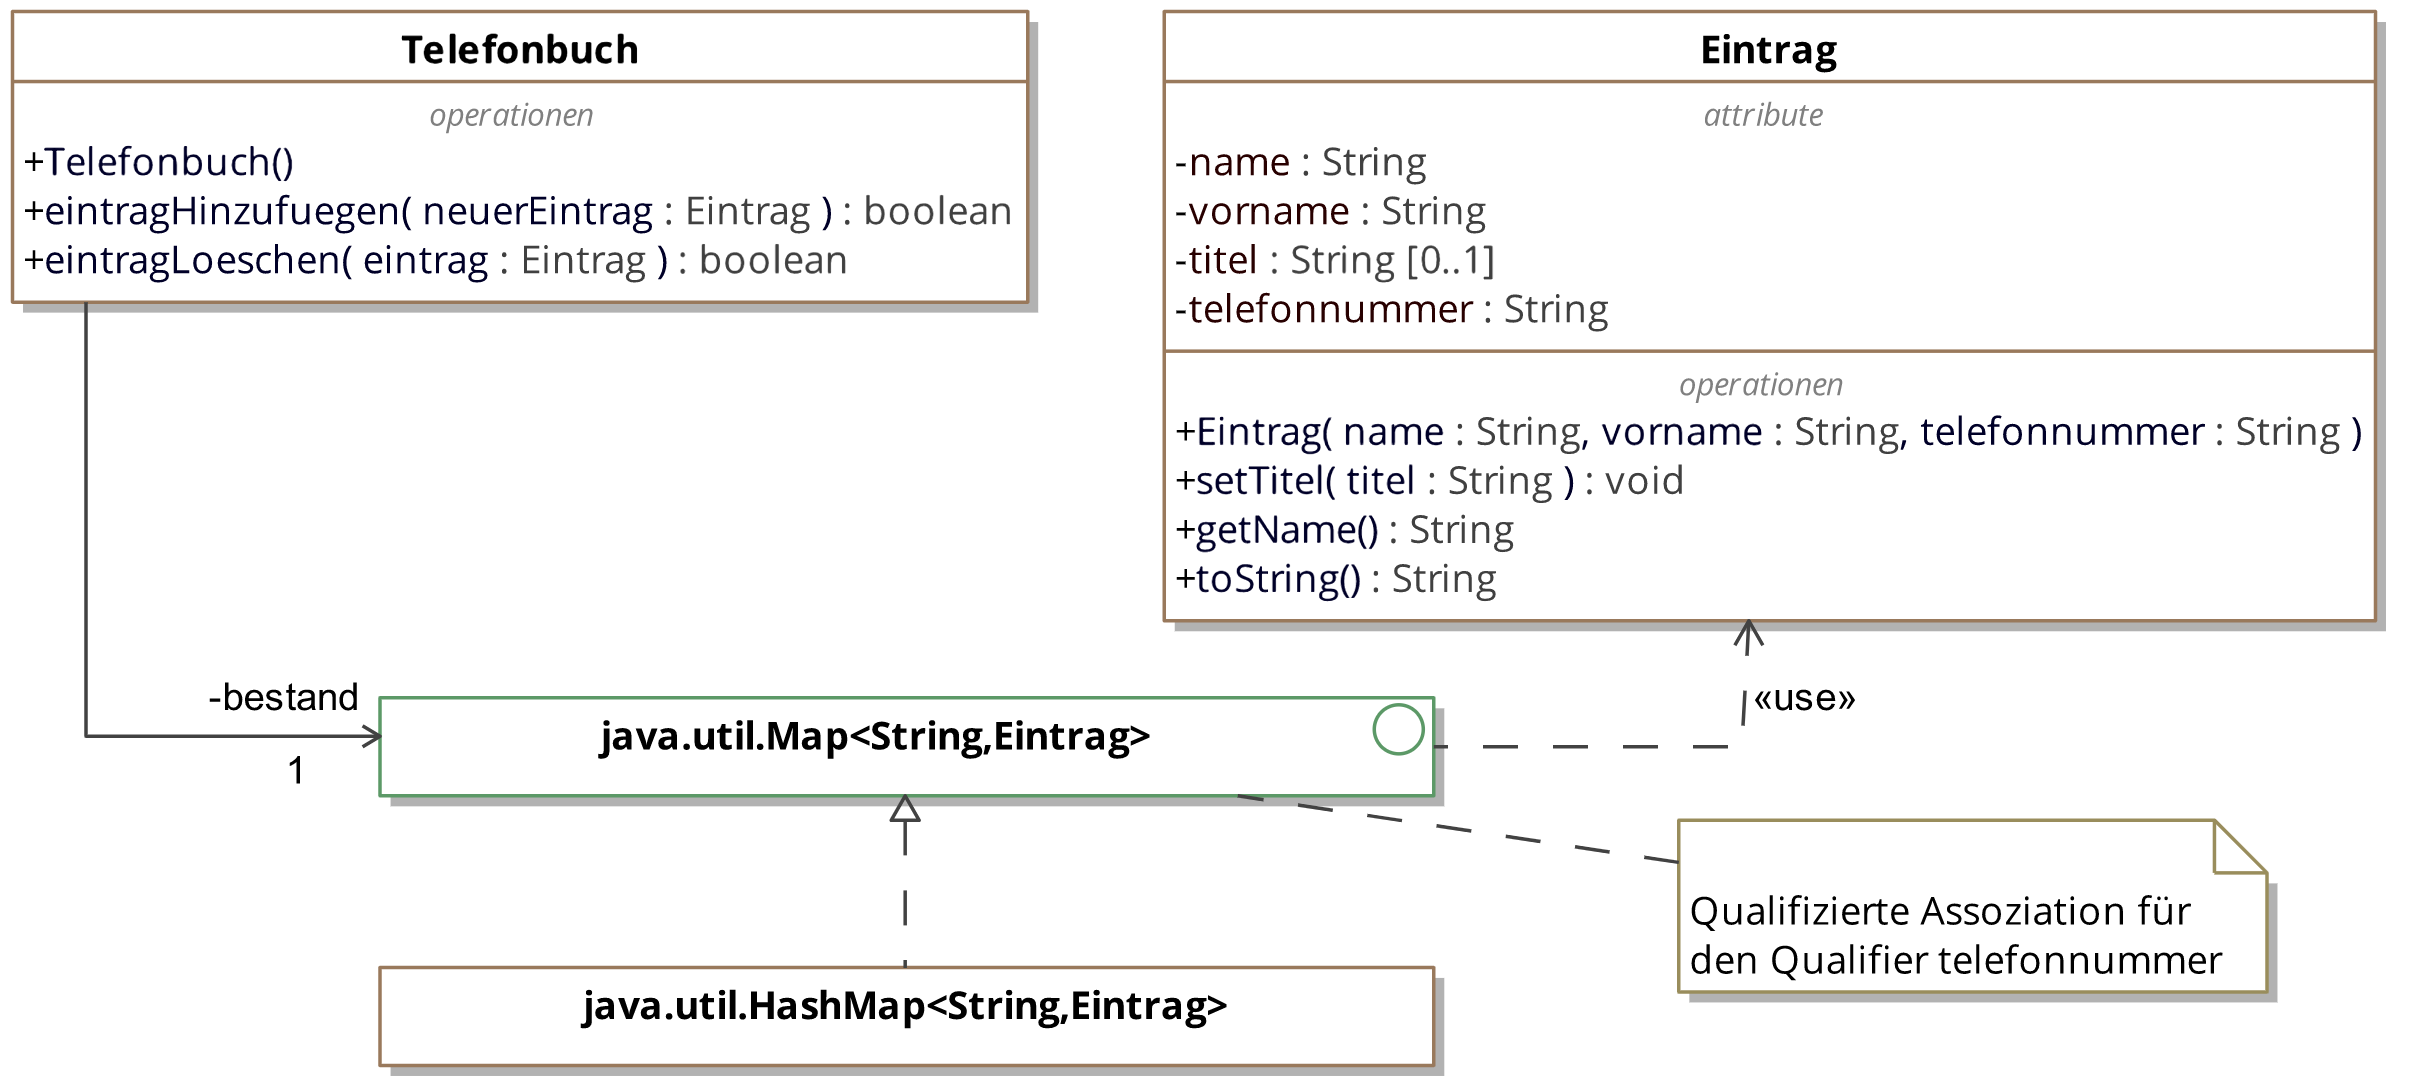
\includegraphics[width=0.75\textwidth]{./Aufgabe13_2c3}
			\end{center}
			\item Zu jedem Namen gibt es beliebig viele Einträge (z.B. Set mit Einträgen)
			\begin{center}
				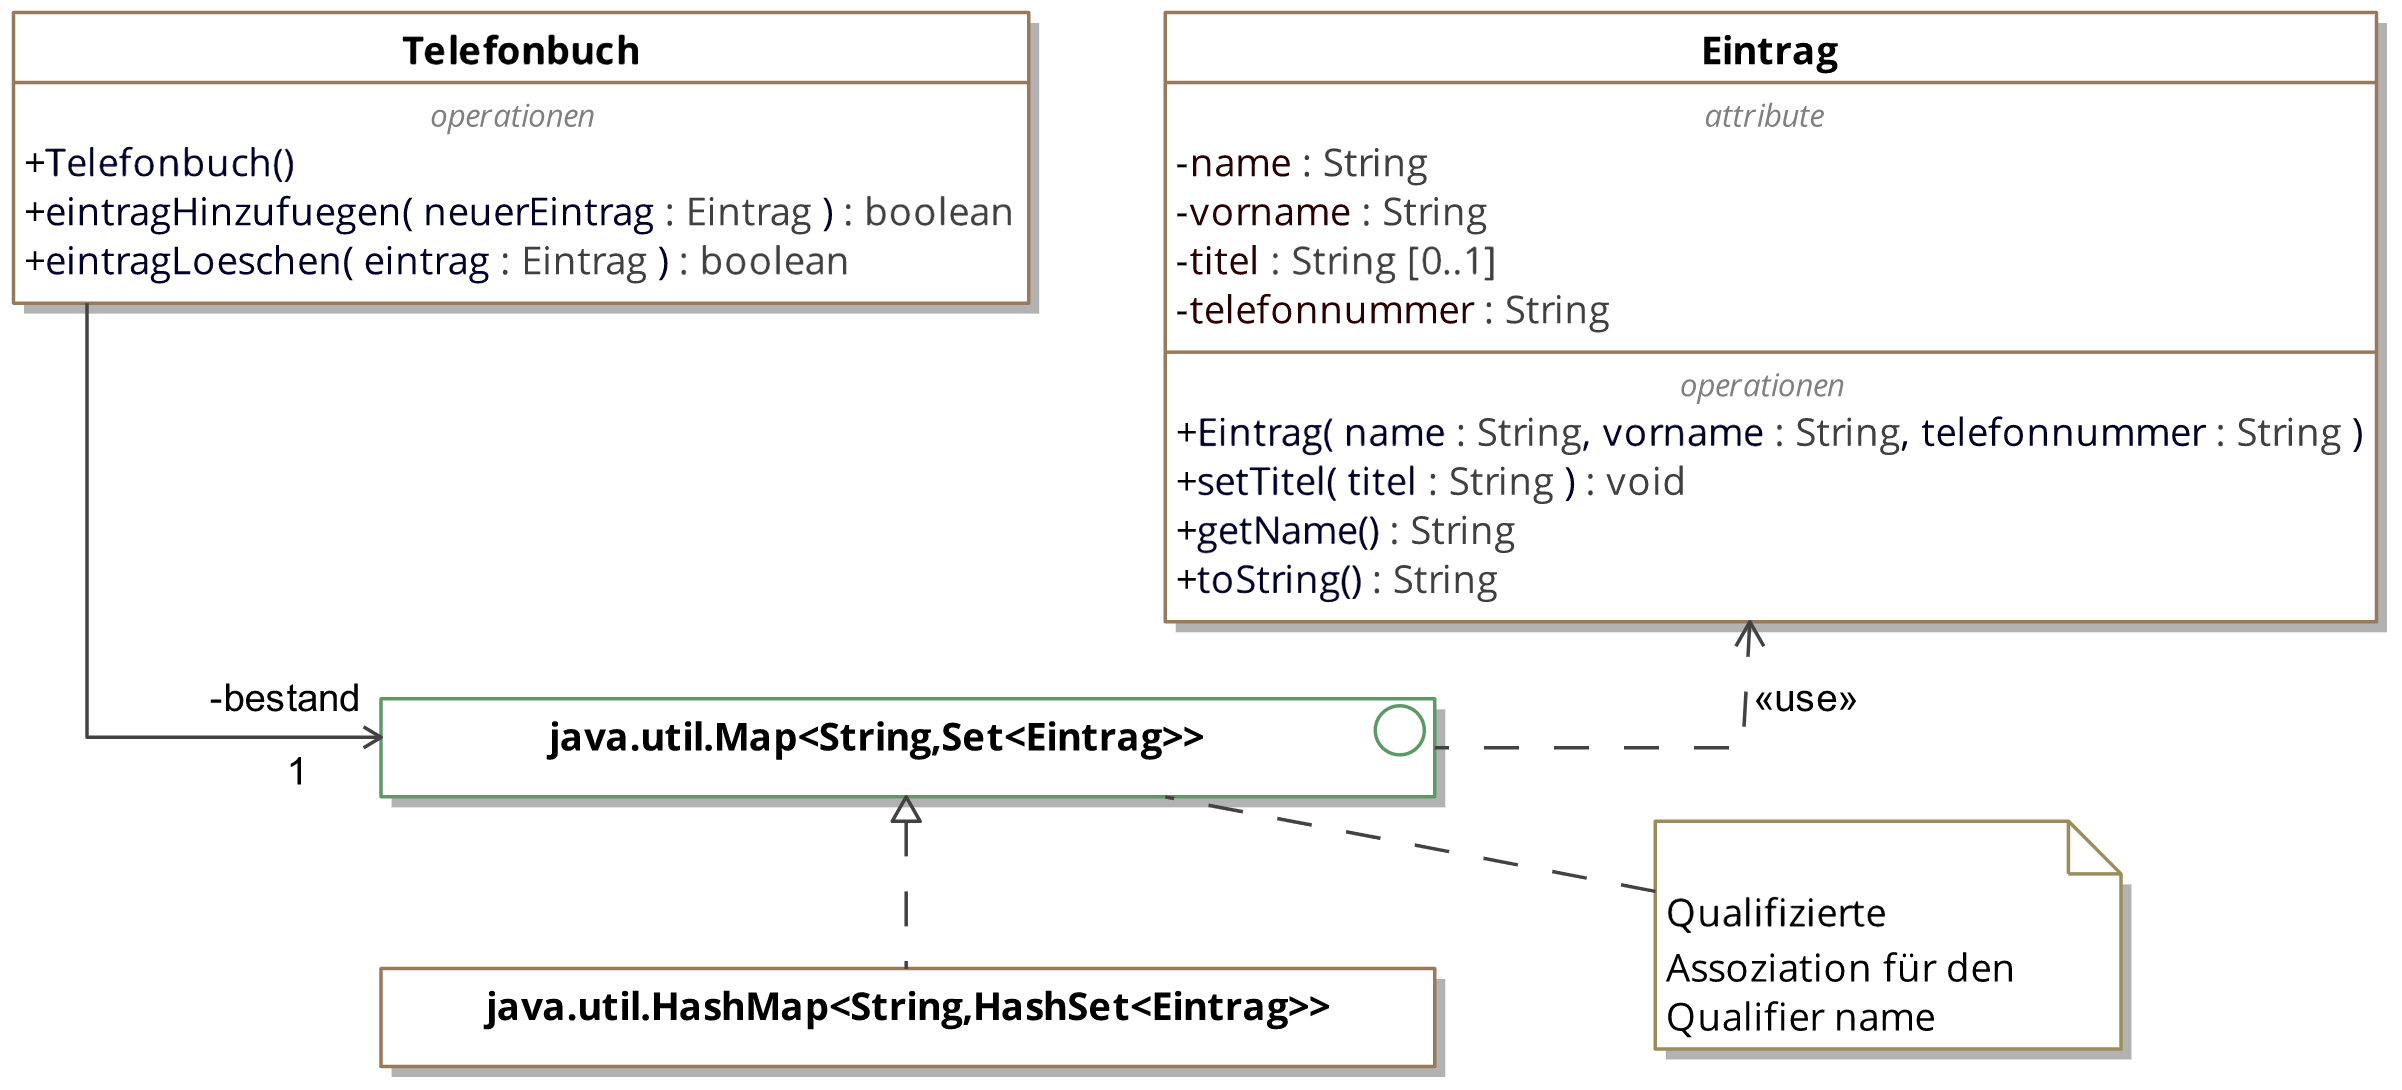
\includegraphics[width=0.75\textwidth]{./Aufgabe13_2c4}
			\end{center}
		\end{itemize}
		\item aUML:
		\begin{center}
			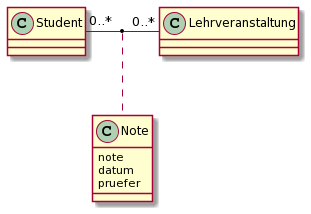
\includegraphics[width=0.5\textwidth]{./Aufgabe13_2d1}
		\end{center}
		dUML:
		\begin{center}
			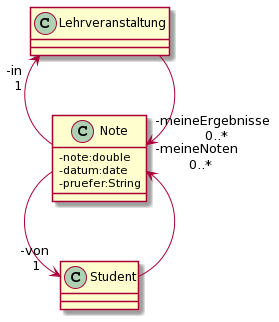
\includegraphics[width=0.5\textwidth]{./Aufgabe13_2d2}
		\end{center}
		\item aUML (Mehrfachvererbung):
		\begin{center}
			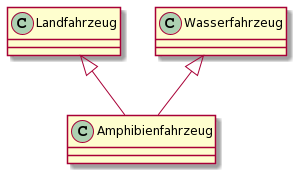
\includegraphics[width=0.5\textwidth]{./Aufgabe13_2e1}
		\end{center}
		dUML (mit Interface):
		\begin{center}
			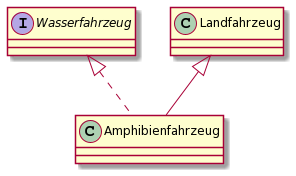
\includegraphics[width=0.5\textwidth]{./Aufgabe13_2e2}
		\end{center}
		\item aUML:
		\begin{center}
			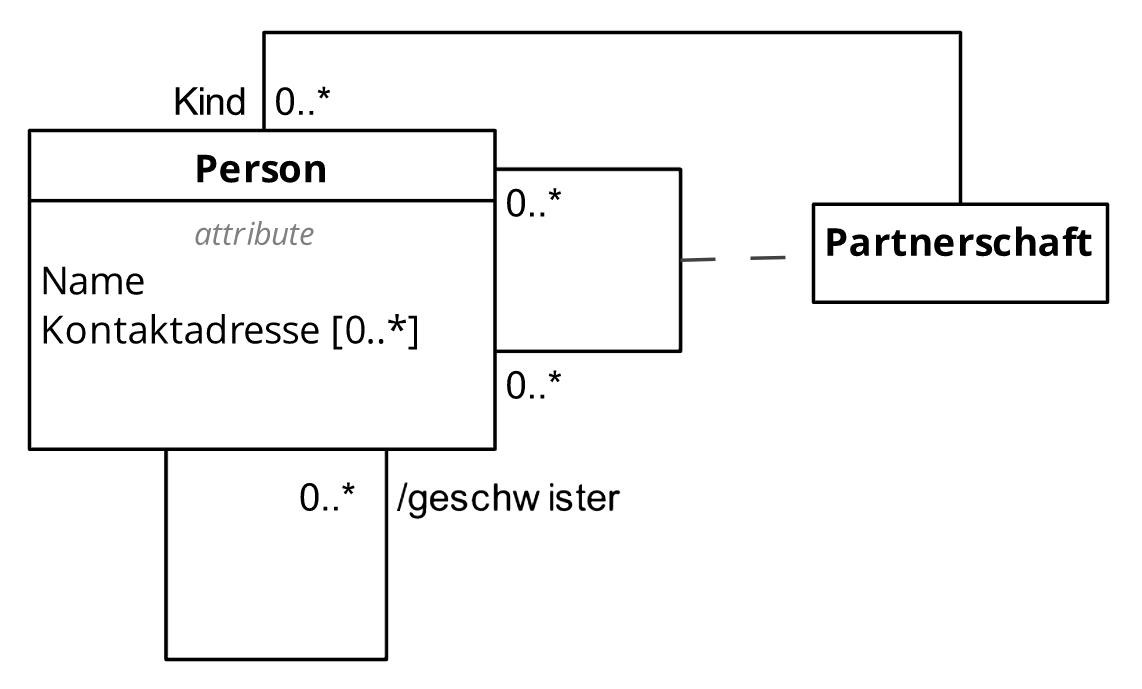
\includegraphics[width=0.75\textwidth]{./Aufgabe13_2f1}
		\end{center}
		dUML:
		\begin{center}
			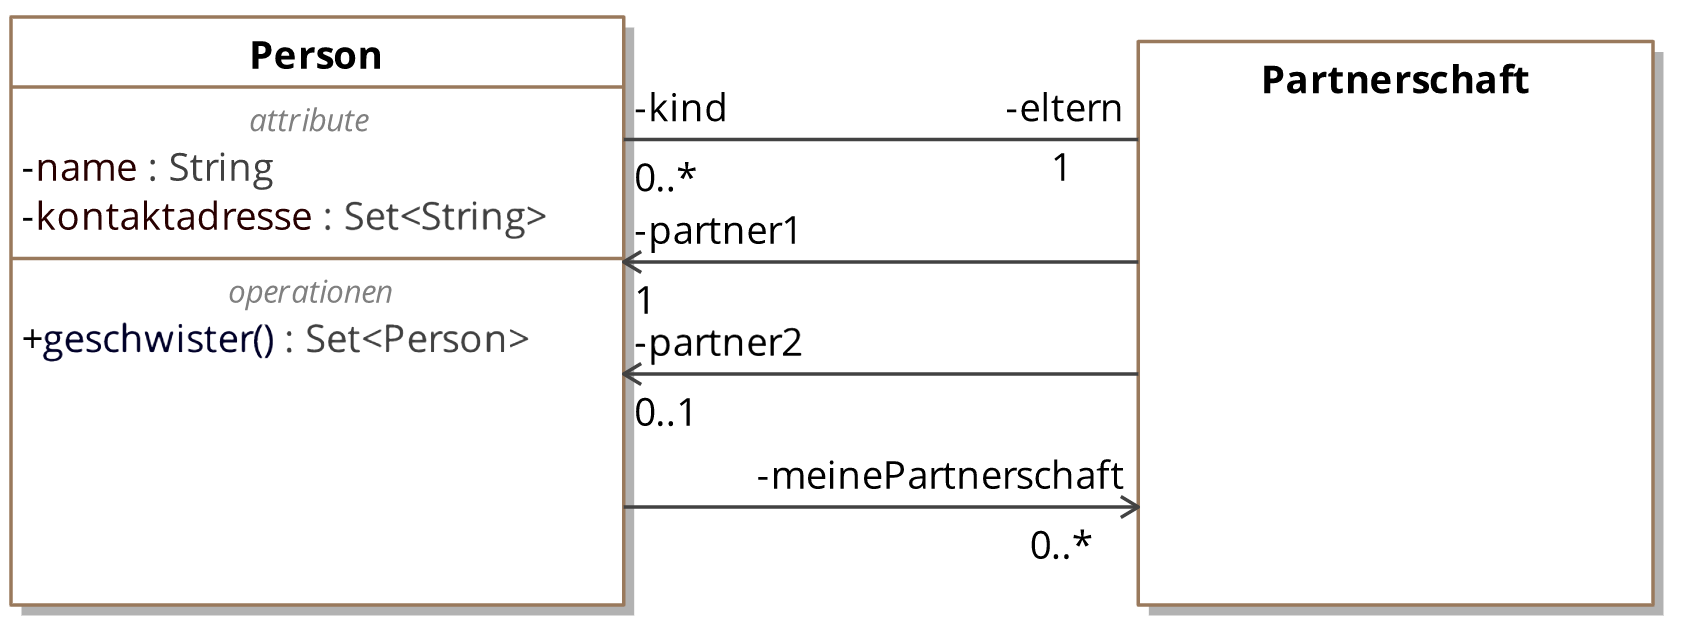
\includegraphics[width=0.75\textwidth]{./Aufgabe13_2f2}
		\end{center}
	\end{enumerate}
	
\end{document}